\documentclass{endm}
\usepackage{endmmacro}
\usepackage{graphicx}
\usepackage{amssymb,amsmath,latexsym}
\usepackage[varg]{pxfonts}
%%%%%% ENTER ADDITIONAL PACKAGES
%\usepackage{graphics}
\usepackage{pst-all}
\usepackage{graphicx}
\usepackage{subfig}
\usepackage{amsfonts}
\usepackage{amssymb} % ADDED
\usepackage{times}
\usepackage{latexsym}
\usepackage{fancybox}
\usepackage{algorithm}
%\usepackage{algorithmic}
\usepackage{algorithmicx}
\usepackage{algpseudocode}
\usepackage{setspace}
\usepackage{courier}
\usepackage{verbatim}
\usepackage{hhline}
\usepackage{etex}
\usepackage{graphicx}
\usepackage{listings}
\usepackage{tikz}
\usetikzlibrary{calc,arrows,automata}
\usetikzlibrary{matrix,positioning,arrows,decorations.pathmorphing,shapes}
\usetikzlibrary{shapes,snakes}
\usepackage{graphicx}
%---------------
\usepackage{mathtools}
\usepackage{booktabs}
\usepackage{hyperref}
\makeatletter
\let\c@author\relax
\makeatother
\usepackage[backend=bibtex,style=alphabetic,
sorting=ynt
]{biblatex}
\addbibresource{sources.bib}
\lstdefinestyle{mystyle}{
    backgroundcolor=\color{backcolour},   
    commentstyle=\color{codegreen},
    keywordstyle=\color{magenta},
    numberstyle=\tiny\color{codegray},
    stringstyle=\color{codepurple},
    basicstyle=\ttfamily\footnotesize,
    breakatwhitespace=false,         
    breaklines=true,                 
    captionpos=b,                    
    keepspaces=true,                 
    numbers=left,                    
    numbersep=5pt,                  
    showspaces=false,                
    showstringspaces=false,
    showtabs=false,                  
    tabsize=2
}


\tolerance=1
\emergencystretch=\maxdimen
\hyphenpenalty=10000
\hbadness=10000


\floatname{algorithm}{Algorithm}


\def\lastname{Please list your Lastname here}

\begin{document}


\begin{frontmatter}

\title{Métodos Numéricos 2019 - Obligatorio 2}

\author{Bruno Figares (4391788-8),}
\author{Adrián Gioda (4954044-5),}
\author{Daniel Martinez (4462694-5),}
\author{Adriana Soucoff (3190794-8)}

\address{Instituto de Matem\'atica y Estad\'istica\\ Facultad de Ingenier\'ia. Universidad de la Rep\'ublica\\ Montevideo, Uruguay}


\begin{abstract}
\setlength{\parindent}{12pt}
Este informe presenta resolución de problemas utilizando distintos métodos y comparando cada uno de ellos, está organizado según tres temas:\\
    - Problema de mínimos cuadardos no lineal(PMCNL) utilizando los métodos de Ecuaciones Normales, descomposición QR y Gauss-Newton, junto a la discusión de ventajas y desventajas de los métodos para este caso.\\
    - Problema de resolver ecuaciones diferenciales ordinarias (EDO) utilizando los métodos de Euler hacia atrás, Euler hacia adelante y Runge-Kutta, se discute ventajas y desventajas.\\
    - Problema de Interpolación utilizando los métodos de interpolación lineal a trozas y Splines Cúbicos, se discute ventajas y desventajas.
\end{abstract}

\begin{keyword}
PMCL, PMCNL, Ecuaciones Normales, Descomposición QR, Gauss-Newton, EDO, Euler, Estabilidad, Runge-Kutta, Interpolación, Lineal a trozos, Splines Cúbicos.
\end{keyword}
\end{frontmatter}

\section{Introdución}\label{intro}
%Ej2
Se presentan dos tablas de mediciones para las funciones no lineales $g_1$ y $g_2$ 


se definen :\\
$g_1(x)=c x^{-p} $ y $g_2(x)=d x^{-q} $

se convierten los problemas a PMCL y se resuelven a través del método de Ecuaciones Normales y método de descomposición QR, al igual que se resuelve de manera directa el PMCNL con el método de Gauss-Newton.

%Ej3
Se busca resolver la ecuación diferencial:
\begin{equation*}
    (PVI):\begin{cases}
        y'(x) = -g_1(x)y + g_2(x) \\
        y(1/2) = 0
    \end{cases}
\end{equation*}
para ello se resuelve de forma analítica (es una ecuación con una solución de forma cerrada), con métodos de Euler (hacia adelante y hacia atrás) y con un método de Runge-Kutta de paso variable (ode45).

%Ej4
Se realiza interpolación de los resultados tanto lineal a trozos como con splines cúbicos.
\section{Metodología}\label{AA}

%Ej2.1
\subsection{PMCNL - Transformación a PMCL}
El modelo de ambas funciones tiene la forma $y = cx^{-p}$. Esta puede transformarse en una relación
lineal aplicando un logaritmo a ambos lados de la expresión de esta forma, $log(y) = log(cx^{-p}) = log(c) + (-p)log(x)$.
Aplicando cambios de variable apropiados, se obtiene la relación lineal $Y = c_2 + c_1X$.

Se busca el vector $C$ de coeficientes que minimizá $||AC - Y||^2_2$,
con $A = \begin{pmatrix}X_1 & 1 \\ \vdots & \vdots \\ X_m & 1 \end{pmatrix}$.
Para esto se deben resolver las ecuaciones normales $A^tAC = A^tY$.

Resolución de las ecuaciones normales:
desarrollamos para el caso de $g_{1}$ es análogo para $g_{2}$ sustituyendo $c$ por $d$ y $p$ por $q$ 

$Y =log(y)$ , $X =log(x)$ , $c_1= log(c)$, $c_2= -p$ \\
siendo $n$ el largo del vector $X$ tenemos las ecuaciones normales
\begin{equation}
\begin{cases}
\sum Y = n * c_1 + c_2 * \sum X \\
\sum X * Y = c_1 * \sum X + c_2 * \sum X^2
\end{cases}
\end{equation}  \\
Siendo \begin{equation*}C=\begin{pmatrix}
          c_1 & \\
          c_2
         \end{pmatrix} \\
\end{equation*}
Resolvemos : $ C=(A^t * A) \setminus  (A^t * Y)$ \\
Finalmente obtenemos:  $c= exp(c_1)$, $p = -c_2$ \\


Aplicación de descomposición QR:
Debido a que el calculo de $A^tA$ esta mal condicionado, se aplica la descomposición QR de $A$.
Teniendo que $A \in \mathcal{M}_{m \times n}$, con $m > n$ tiene rango completo (sus columnas son LI),
por el teorema 4.3.1 de los apuntes se tiene que existen matrices $Q \in \mathcal{M}_{m \times m}$,
$R \in \mathcal{M}_{m \times n}$ tales que $A = QR$. Con $Q$ ortogonal
y $R$ triangular superior de la forma  \begin{equation*} \begin{pmatrix} R_1 \\ 0 \end{pmatrix}\end{equation*} con $R_1 \in \mathcal{M}_{n \times n}$.

Sustituyendo $A$ por $QR$, el problema de minimizacion se torna $min ||QRC - Y||^2_2$.
Separando a $Q$ en dos partes $[Q_1 Q_2]$ tal que $Q_1 \in \mathcal{M}_{m \times n}$ y
$Q_2 \in \mathcal{M}_{m \times (m-n)}$ y operando, se llega al problema de minimizacion $min ||R_1C - Q_1^tY||^2_2$
cuya solución proviene del sistema de ecuaciones $R_1C = Q_1^tY$, que como $R_1$ es triangular superior se resuelve con
sustitución hacia atrás.

% Falta mostrar las matrices A, Y, Q1, R1 y la solucion C. Ademas hay que poner las graficas. %

%Ej2.2
\subsection{PMCNL - Resolución por Gauss-Newton}
Otra manera de resolver el problema sin tener que utilizar logaritmos es a través del uso de los polinomios de taylor lineales. Para esto, para ajustar los puntos $X_i,Y_i$, con $ i \in \{1,..,n\}$

\begin{align*}
&F(c,p) =||X_{c,p} - Y||^2_2 \\
&X_{c,p} = c*X_i^p \forall i \in \{1,..n\}
\end{align*}

Con este problema nuevo, asumimos que estamos cerca de una solución y linealizamos el problema a través del polinomio de taylor de orden 1, con la posibilidad de obtener una solución con un error acotado por el cuadrado de la distancia de la solución inicial $k$
\begin{equation*}
F_k = ||  F(k) + \Delta F(k)\Delta_{c,p} - Y + o(\Delta_{c,p}^2)||^2_2\\
\end{equation*}
Haciendo los siguientes cambios de variable obtenemos una secuencia de PMCL que podemos resolver y encontrar soluciones progresivamente mejores
\begin{align*}
&F_{k_i} \simeq || F(k_i) + \Delta F(k_i)\Delta_{c,p} - Y||^2_2\\
&Y_{k_i} = Y - F(k_i) \\
&k_{i+1} = k_i + \min_{\Delta_{c,p}} || \Delta F(k_i)\Delta_{c,p} - Y_{k_i} ||^2_2
\end{align*}



%Ej3.1
\subsection{EDO - Resolución Analítica}
Se resuelve analíticamente en primer lugar a fin de poder evaluar la solución provista por distintos métodos numéricos.
En la parte 2 se vio que $g_1(x) = cx^{-2}$ y $g_2(x) = dx^{-3}$ con $c,d \in \mathbb{R}$.
La ecuación diferencial es entonces:
\begin{equation}
    y' + \frac{c}{x^2}y = \frac{d}{x^3}
\end{equation}
Solución de la homogénea:
 \begin{equation*}
\begin{cases}
    y' + \frac{c}{x^2}y = 0 \\
    y_h = exp(-\int cx^{-2}dx) \\
    y_h = ke^{c/x}
\end{cases}
\end{equation*}
Variación de constantes:
Se escribe la función $y$ como $y = k(x)e^{c/x}$. La idea es obtener la expresión de $k(x)$.
Se deriva $y$: $y' = k'(x)e^{c/x} + k(x)\left(-\frac{c}{x^2}e^{c/x}\right)$
Sustituyendo en la EDO, se cancelan dos términos y se despeja $k'(x)$. Integrando la expresión resultante se obtiene $k(x)$.
\begin{equation}
    k(x) = \int \frac{d}{x^3}e^{-c/x}dx
\end{equation}
Aplicando integración por partes con $u = \frac{d}{x}$, $du = -\frac{d}{x^2}$, $v = e^{-c/x}$ y $dv = \frac{c}{x^2}e^{c/x}$ se llega a:
\begin{equation}
    k(x) = \frac{1}{c}\left( \frac{d}{x}e^{-c/x} + C_1 + \frac{d}{c}\int e^{-c/x}\frac{c}{x^2}dx \right)
\end{equation}
Aplicando integración por sustitución con la misma $v$ y $dv$ se tiene que:
\begin{equation}
    k(x) = \frac{1}{c}\left( \frac{d}{x}e^{-c/x} + C_1 + \frac{d}{c}e^{-c/x} + C_2 \right) =
    \frac{d}{c}e^{-c/x}\left( \frac{1}{x} + \frac{1}{c} \right) + k
\end{equation}
Finalmente se llega a la expresión de $y$:
\begin{equation}
    y(x) = \frac{d}{c^2} + \frac{d}{cx}+ ke^{c/x}
\end{equation}
Usando la condición inicial $y(1/2) = 0$ se halla que $k = -\frac{d}{c}\left( \frac{1}{c} + 2 \right)e^{-2c}$.

%Ej3.2
\subsection{EDO - Métodos de Euler}

% Euler hacia adelante %
En el método de Euler hacia adelante estima la derivada en el punto $x_{n}$ mediante el cociente entre la diferencia de los pasos consecutivos $y_{n+1}$ e $y_{n}$ y el paso $h$. Es un método explícito.\\
$y'(x_{n}) = \frac{y_{n+1} - y_n}{h} = f(x_{n},y_{n})$\\
despejando:
$y_{n+1} = y_n + hf(x_{n},y_{n})$ \\

Entonces se tiene la iteración:
\begin{equation*}
\begin{cases}
    y_{k+1} = y_k + hf(x_{k},y_{k}) \\
    y_0 = y_{inicial}
\end{cases}\\
\end{equation*}
con $x_{k} = x_{0} + kh$ con  $h>0$ fijo \\
Para nuestro caso tenemos:
\begin{align*}
    y_{k+1} &= y_k + hf(x_{k},y_{k}) \\
    &= y_k + h\left( \frac{d}{x_{k}^3} - \frac{c}{x_{k}^2}y_{k} \right)
\end{align*}


El método de Euler hacia atrás estima la derivada en el punto $x_{n+1}$ imponiendo $y'(x_{n+1}) = \frac{y_{n+1} - y_n}{h} = f(x_{n+1},y_{n+1})$.
Entonces se tiene la iteración:
\begin{equation*}
\begin{cases}
    y_{k+1} = y_k + hf(x_{k+1},y_{k+1}) \\
    y_0 = y_{inicial}
\end{cases}
\end{equation*}
Debido a que $y_{k+1}$ aparece en ambos lados de la ecuación, este es un método implícito. Sin embargo, si
$f$ es lineal en $y$, se puede obtener una formulación explicita.

En este caso, la EDO a resolver es $y' = f(x,y) = \frac{d}{x^3} - \frac{c}{x^2}y$. Dado que $f$ es lineal en $y$, se desarrolla
la formulación explicita para $y_{k+1}$.
\begin{align*}
    y_{k+1} &= y_k + hf(x_{k+1},y_{k+1}) \\
    &= y_k + h\left( \frac{d}{x_{k+1}^3} - \frac{c}{x_{k+1}^2}y_{k+1} \right)
\end{align*}
Despejando $y_{k+1}$ se obtiene:
\begin{equation}
    y_{k+1} = \frac{y_k + \frac{hd}{x_{k+1}^3}}{1 + \frac{hc}{x_{k+1}^2}}
    % otra forma menos compacta: %
    %y_{k+1} = \left( \frac{1}{1 + \frac{hc}{x_{k+1}^2}} \right) \left( y_k + \frac{hd}{x_{k+1}^3}\right)%
\end{equation}.\\

Estabilidad numérica \\
Un método es numéricamente estable si dada la solución de la ecuación de diferencias $y_k$ dada por el método y dicha solución
calculada por la maquina $\overline{y}_k$, su diferencia $\overline{E}_k = \overline{y}_k - y_k$ se mantiene acotada al crecer k.

La región de estabilidad asociada a un método dado se define como los puntos $z = hq$ del plano complejo tales que 
la sucesión ${y_n}$, generada por el método numérico aplicado a el problema test, se mantiene acotada con $n$.
El problema test se define como el problema de valores iniciales:
\begin{equation*}
\begin{cases}
    y' = qy \\
    y(0) = 1
\end{cases}
\end{equation*}

Euler hacia adelante:
Aplicando el método al problema test se tiene que:
$y_{n+1} = y_n + h(qy_n) = (1 + hq)y_n$
Desarrollando la recurrencia se llega a que:
$y_{n+1} = (1 + hq)\times (1 + hq)y_{n-1} = \dots = (1 + hq)^{n+1}y_0$
Para que $\{y_n\}$ este acotado, $z = hq$ debe ser tal que $|1 + hq| <1$, dado que $|y_n| = |1 + hq|^n|y_0|$
Por tanto, la región de estabilidad en el plano complejo esta dada por $R_{euler} = \{hq \in \mathbb{C}:|1 + hq| \leq 1\}$

Euler hacia atrás:
Se aplica el método al problema test para obtener:
$y_{n+1} = y_n + h(qy_{n+1}) \Rightarrow y_{n+1}(1 - hq) = y_n \Rightarrow y_{n+1} = \frac{y_n}{1 - hq}$
Se desarrolla la recurrencia hasta $y_0$
$y_{n+1} = \frac{y_n}{1 - hq} = \frac{y_{n-1}}{(1 - hq)^2} = \dots = \frac{y_{n-1}}{(1 - hq)^{n+1}}$
Para que $\{y_n\}$ este acotado, $z = hq$ debe ser tal que $\frac{1}{|1 - hq|} \leq 1 \iff |1 - hq| \geq 1$
Por lo que la región de estabilidad en el plano complejo esta dada por $R_{EA} = \{hq \in \mathbb{C}:|1 - hq| \geq 1\}$

%TODO
% Gráficas y explicación de región de estabilidad para euler FW y BW

%Ej3.3
\subsection{EDO - Implementación de los Métodos de Eueler}

Ver código.

%Ej3.4
\subsection{EDO - Método de Runge-Kutta}
Los métodos de Runge-Kuta calculan el valor de un punto $y_{n+1}$ a partir del punto anterior $y_n$ y de
un promedio ponderado de las derivadas en distintos puntos en el intervalo $[x_n, x_{n+1}]$.
El usado para esta sección es el implementado por la función ode45 de Octave.
Este es un método de 6 etapas de orden 5 y funciona de la siguiente manera:
Empezando en el punto $(x_n,y_n)$ con pendiente $s_1 = y' = f(x_n,y_n)$ y un paso $h$ de tamaño apropiado,
se busca computar $y_{n+1}$ en el punto $x_{n+1} + h$.
Usando "Euler hacia adelante" con la pendiente $s_1$ y una fracción del paso $h$ se obtiene un segundo punto
con el cual se calcula la pendiente $s_2$. Este proceso se repite hasta conseguir $s_6$.
Mediante un promedio ponderado entre las 6 pendientes se calcula $y_{n+1}$
Se calcula una ultima pendiente $s_7$ en $(x_{n+1},y_{n+1})$ que servirá para calcular una estimación
del error que sera usado para decidir el paso $h$ para el calculo del siguiente punto.

La función ode45 produce una sucesión de puntos $(x_n,y_n)$ que parecen ser demasiado espaciados como se vera
en las gráficas de la sección siguiente. Debido a esto, puede necesitarse un interpolador para poder crear una
gráfica mas suave en Octave. Esto se presentará en Interpolación.


%Ej4.1
\subsection{Interpolación Lineal a Trozos}

%TEORICO INTERPOLACION lineal a trozos
El problema a resolver es encontrar una función $f(x)$ desconocida a partir de un conjuntos de puntos que son datos: $ \left \{ (x_i,y_i): i=0,...,n \right \} $ tales que $f(x_i) =y_i$ \\
El objetivo es encontrar buenas aproximaciones de  $f(x)$ imponiendo que esta aproximación pase por todos los puntos dato.

Para el caso de interpolación lineal a trozos lo que se hace es unir los puntos que son dato trazando una recta para cada par de puntos consecutivos, para ello se utiliza la ecuación de la recta, la recta es válida en el intervalo $\left [ x_i,x_{i+1} \right ]$\\
$y=\frac{y_{i+1}-y_i}{x_{i+1}-x_i}(x-x_i)+y_i$\\

considerando $h$ la distancia entre los $x_i$ el error es $O(h^{2})$

%Ej4.2
\subsection{Interpolación con Splines Cúbicos}

%TEORICO INTERPOLACION SPLINES

Interpolación con splines cúbicos une cada par de punto de los dados con un polinomio cúbico $s_i(x)$   (a diferencia con lineal a trozos que uníamos los puntos con rectas).\\
A estos polinomios se impondrá los extremos por los puntos del intervalo y además que tenga una pendiente y concavidad tal que se solapen con la pendiente y concavidad del próximo polinomio, el objetivo es obtener una curva dos veces derivable en todos los puntos.
Se le llama Spline a un polinomio interpolante cúbico a trozos con derivadas primeras y segundas continuas.
Dos splines de intervalos consecutivos quedan relacionados por las siguientes ecuaciones:\\
- $s_i(x_i) = y_{i-1} \  \  \ 1\leq  i \leq n$\\
- $s_{i-1}(x_i) = y_{i} \  \  \ 1\leq  i \leq n$\\
- $s'_{i-1}(x_i) = s'_{i}(x_i) \  \  \ 1\leq  i \leq n$\\
- $s''_{i-1}(x_i) = s''_{i}(x_i)` \  \  \ 1\leq  i \leq n$\\

cada spline se puede ver como un polinomio cúbico a trozos de Hermite, de esta forma entre cada par de puntos consecutivos tenemos un polinomio cúbico con 4 parámetos, para n puntos tenemos un total de 4n incógnitas.
\section{Estudio experimental}
\subsection{Mínimos Cuadrados}
Las funciones son $g_1(x)=c x^{-p} $ y $g_2(x)=d x^{-q} $ con $c,d \in \mathbb{R}$ y $p,q \in \mathbb{Z^+}$
Los errores se calculan como $||Y_{calc} - Y ||^2_2$, donde $Y_{calc} = [cx_1^{-p} \dots cx_{16}^{-p}]^t$ con $p$ entero.
\begin{table}[h!]
    \begin{center}
      \caption{Resultados mínimos cuadrados.}
      \label{tab:table1}
      \begin{tabular}{c|c|c|c|c|c|c|c|c} % <-- Changed to S here.
        \textbf{Método} & \textbf{c} & \textbf{p} & \textbf{error $g_1$} & \textbf{d} & \textbf{q} & \textbf{error $g_2$} \\
        \hline
        Ecs. Normales & 0.96140 & 1.96810 $\approx 2$ & 0.14807 & 1.9598 & 3.0175 $\approx 3$ & 0.43089 \\
        Descomp. QR   & 0.96140 & 1.96812 $\approx 2$ & 0.14807 & 1.9598 & 3.0175 $\approx 3$ & 0.43089 \\
        Gauss-Newton  & 0.96750 & 2.01928 $\approx 2$ & 0.14298 & 1.9949 & 3.0063 $\approx 3$ & 0.25379 \\
      \end{tabular}
    \end{center}
  \end{table}
\clearpage
Debido a que Ecuaciones Normales y Descomposición QR tienen coeficientes iguales, se adjunta solo un set de gráficas para estos.
\begin{figure}%
    \centering
    \subfloat[Visualización exponencial]{{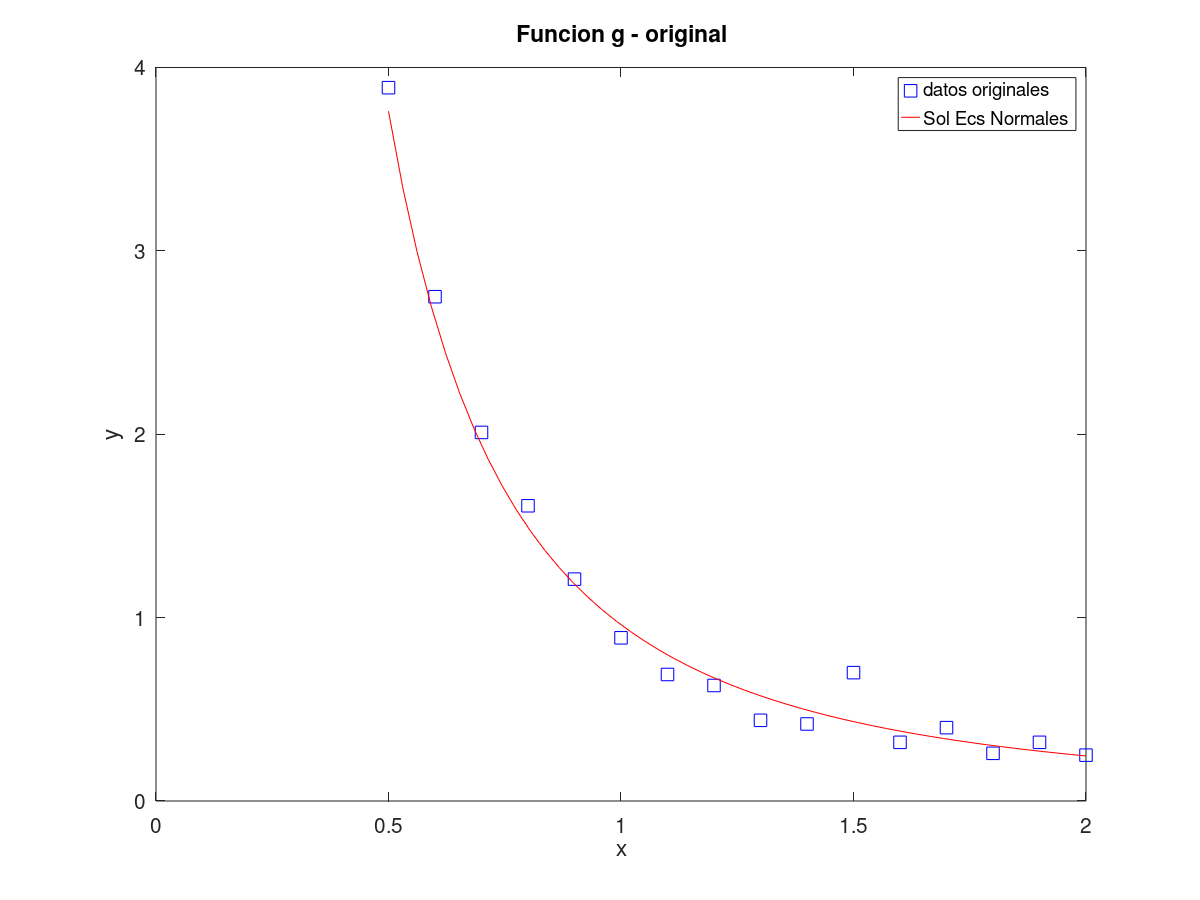
\includegraphics[width=6.25cm]{eng1expmc.png} }}%
    \qquad
    \subfloat[Visualización lineal]{{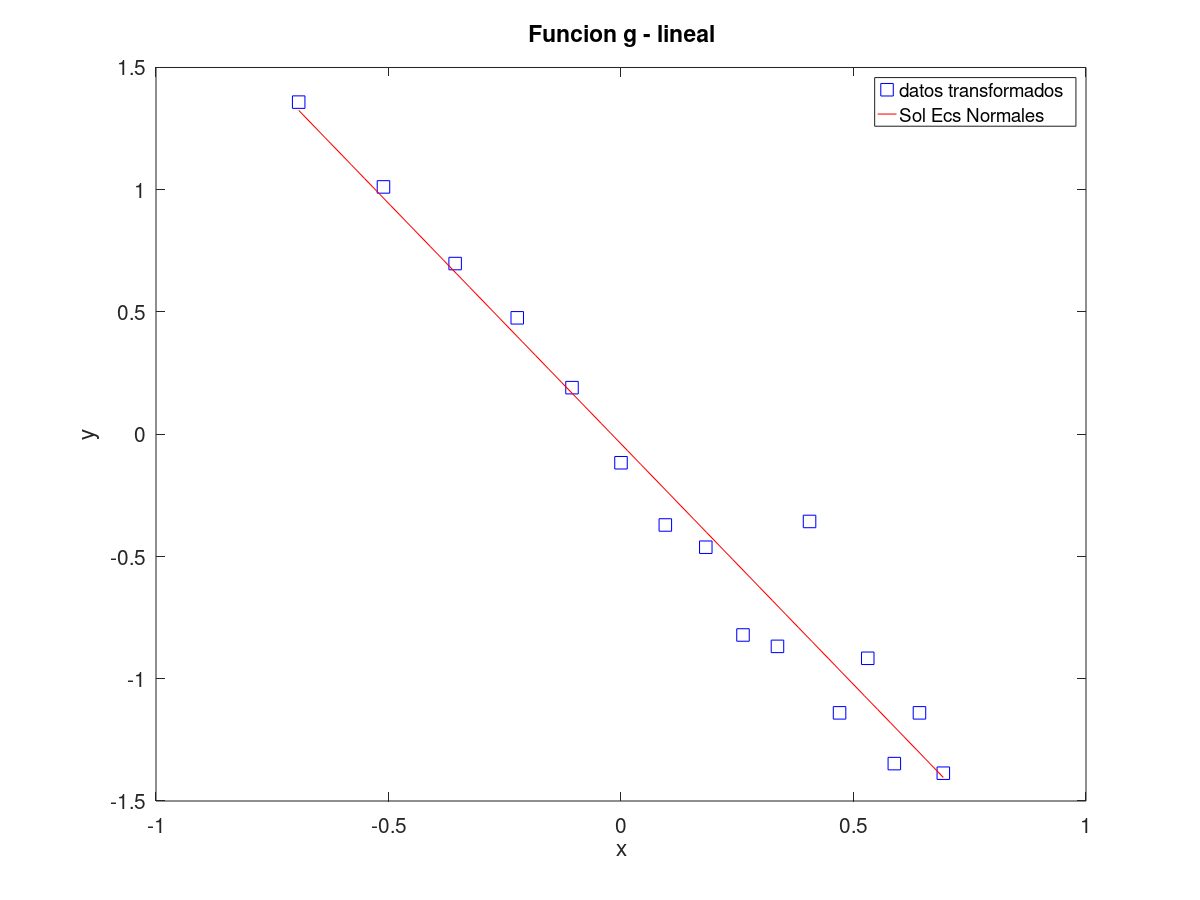
\includegraphics[width=6.25cm]{eng1linealmc.png} }}%
    \caption{Visualización de la función g1 exponencial y lineal por método de ecuaciones normales}%
    \label{fig:example}%
\end{figure}

\begin{figure}%
    \centering
    \subfloat[$g1(x)$]{{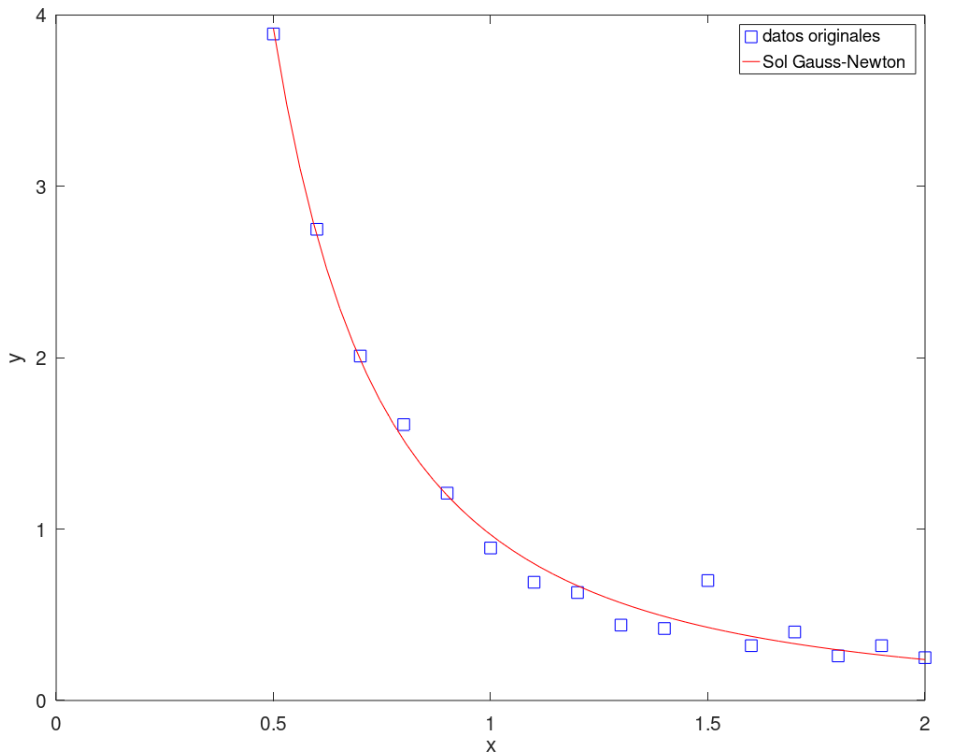
\includegraphics[width=6.25cm]{g1mc.png} }}%
    \qquad
    \subfloat[$g2(x)$]{{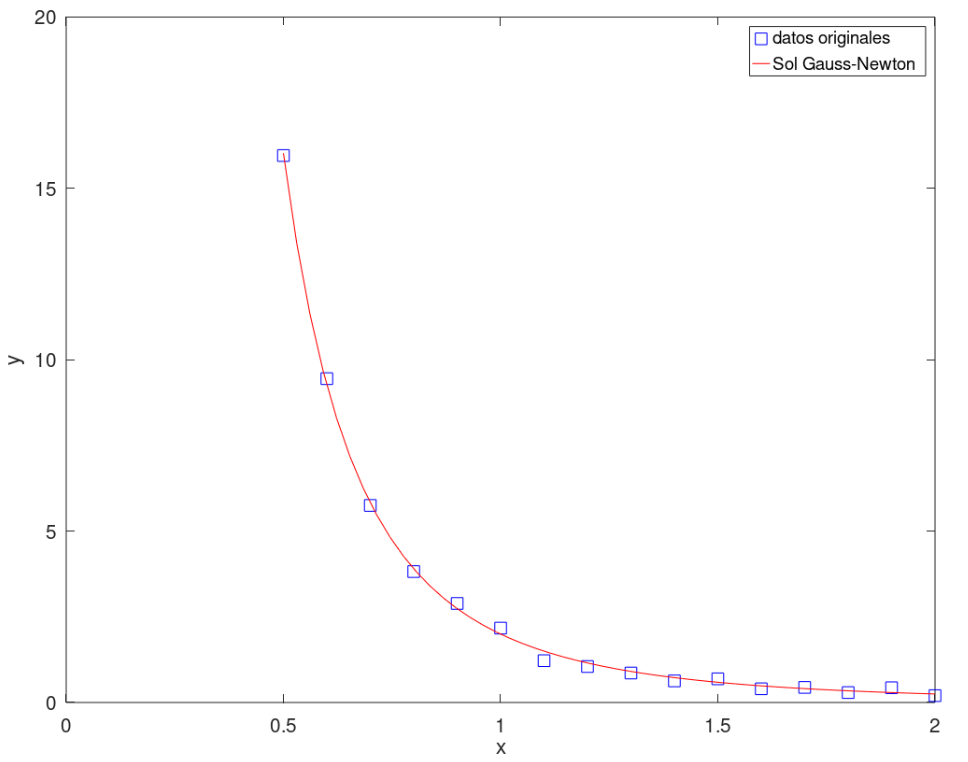
\includegraphics[width=6.25cm]{g2mc.png} }}%
    \caption{Ajuste por mínimos cuadrados de las funciones $g1$ y $g2$ por método de Gauss Newton}%
    \label{fig:example}%
\end{figure}

\subsection{Ecuaciones Diferenciales}
Usando los valores de los coeficientes dados por Gauss-Newton (que obtuvo el menor error), se construyen las gráficas
con la solución de la ecuación diferencial mediante los métodos de Euler y Runge-Kutta con ode45.
Para los métodos de Euler se eligió un paso $h = 0.01$ de forma demostrativa. Este paso da lugar a un error apreciable en
la solución, que sin embargo es acotado y por tanto dentro de la región de estabilidad tal como se ve en la figura \ref{fig:error_euler}.
\begin{figure}
    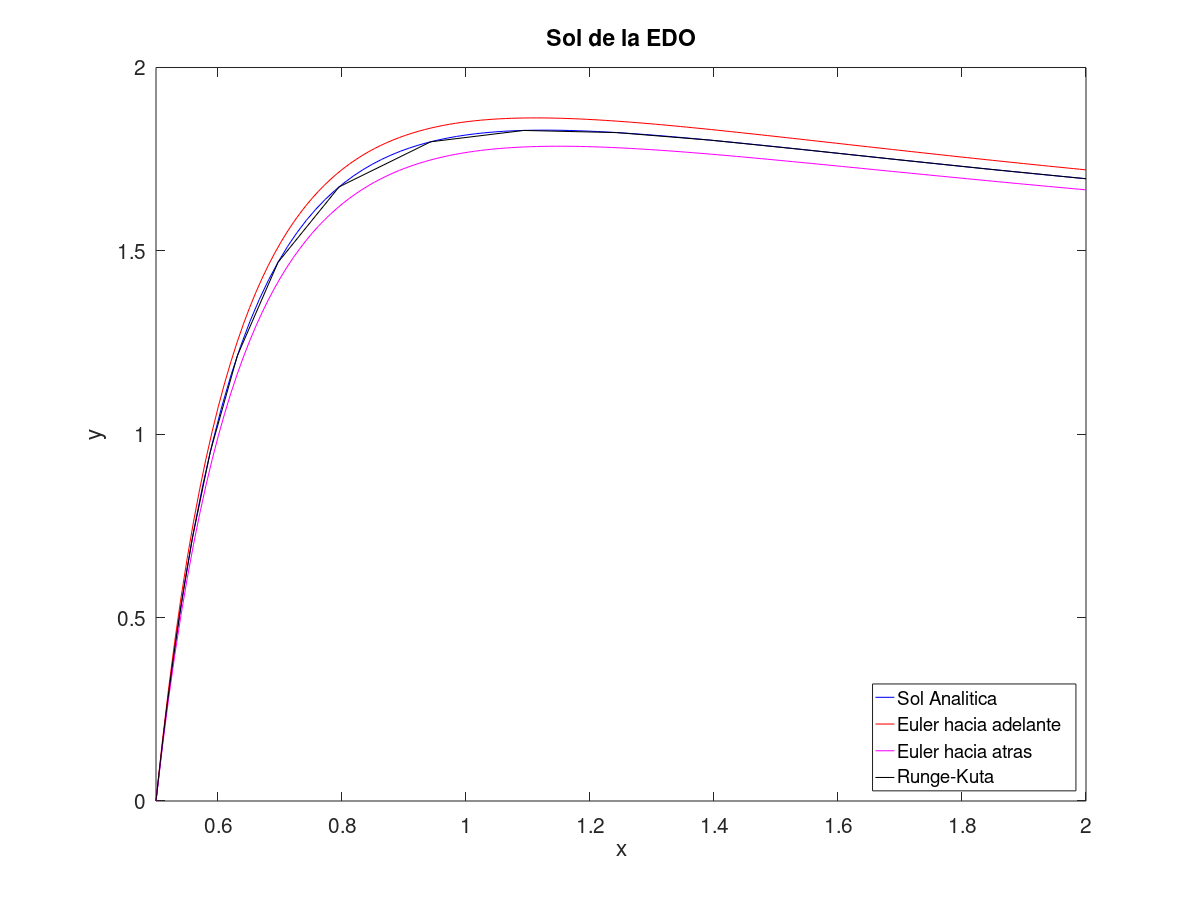
\includegraphics[width=\linewidth]{ecdif.png}
    \caption{Gráficas de los distintos métodos de resolución de ODEs.}
    \label{fig:ecdif}
\end{figure}

\begin{figure}
    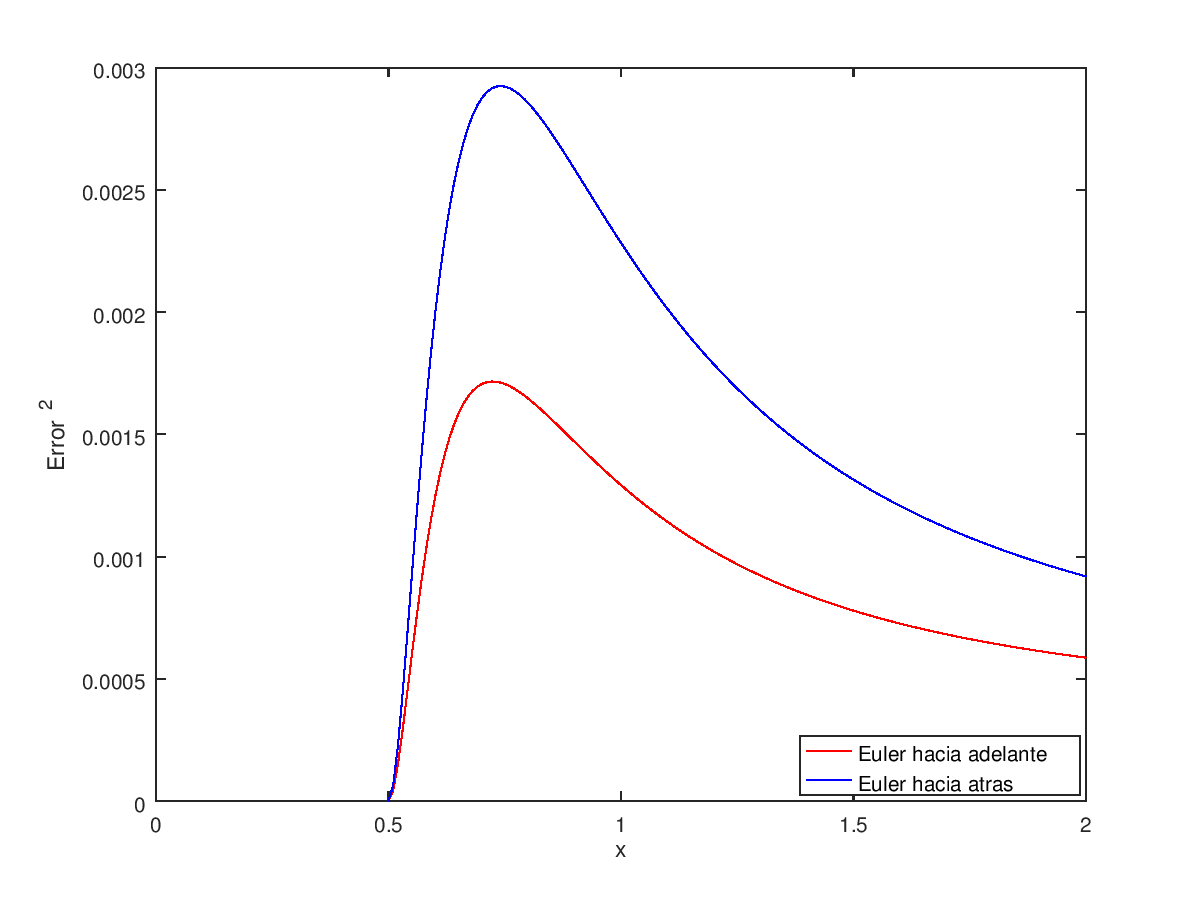
\includegraphics[width=\linewidth]{error_euler.png}
    \caption{Evolución de $(y_{analitica} - y_{euler})^2$.}
    \label{fig:error_euler}
\end{figure}

%\begin{figure}%
%    \centering
%    \subfloat[Ajuste por métodos lineales y ode45]{{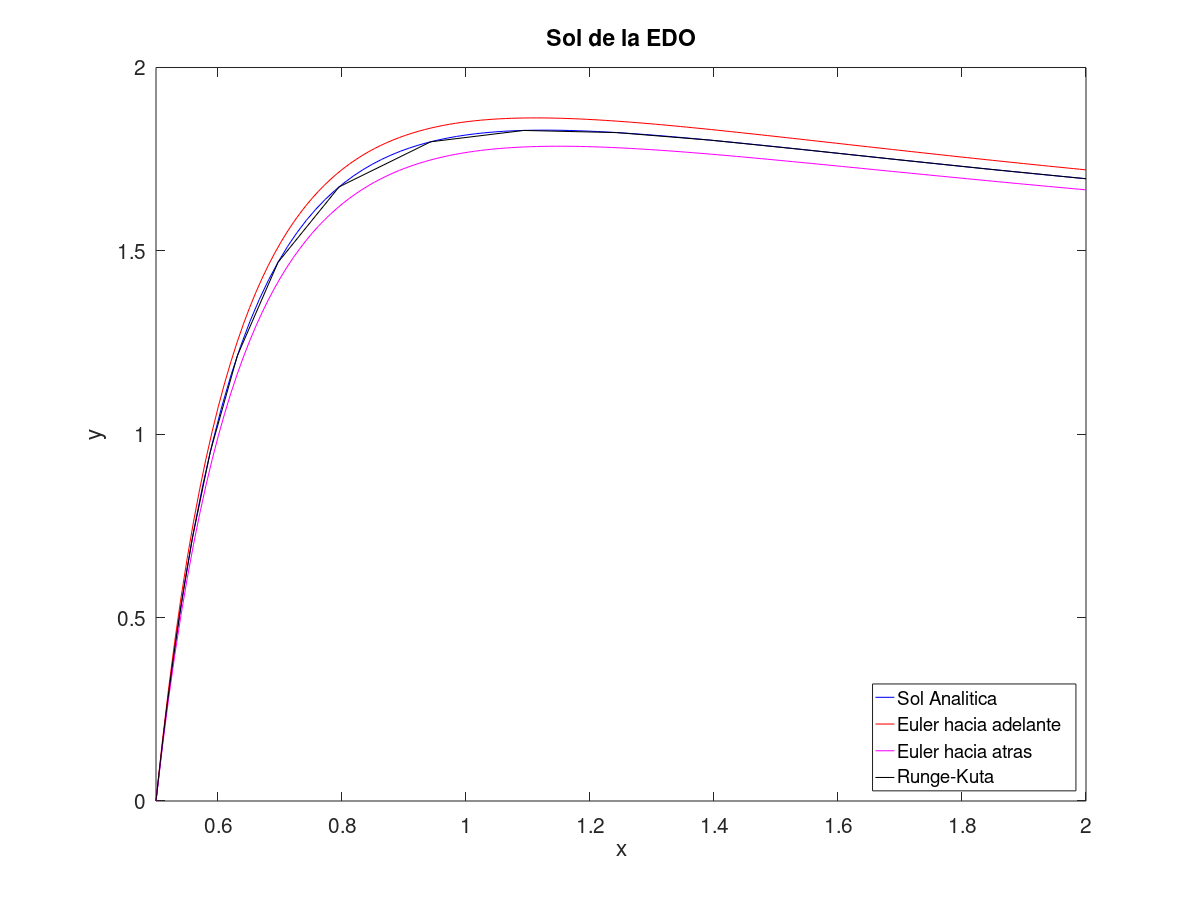
\includegraphics[width=6.25cm]{ecdif.png} }}%
%    \qquad
%    \subfloat[Resultados de interpolación de ode45, lineal y spline cúbica]{{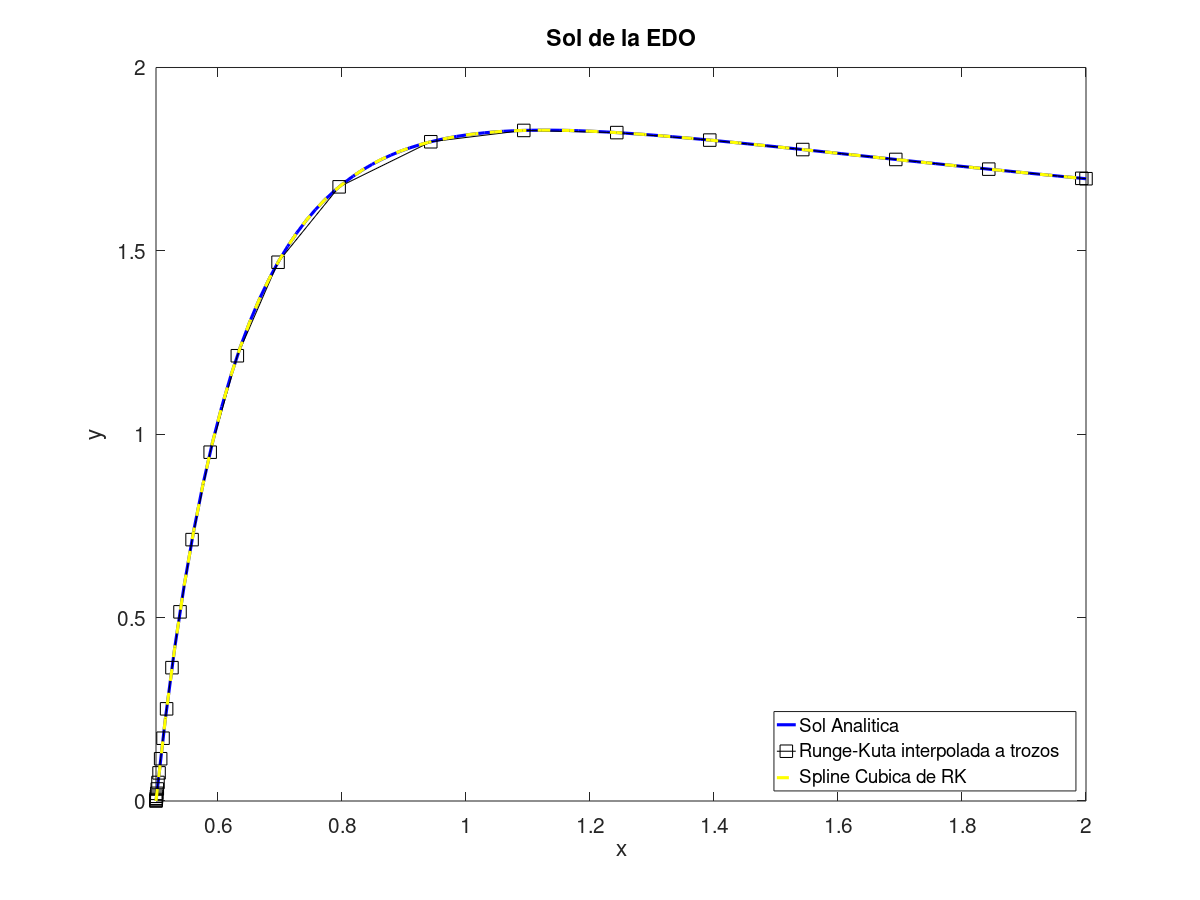
\includegraphics[width=6.25cm]{interpol.png} }}%
%    \caption{}
%    \label{fig:example}%
%\end{figure}

\subsection{Interpolación}



\clearpage
\section{Conclusiones}\label{Conclusiones}

%Ej2.3
\subsection{Comparación - PMCNL}
Los métodos todos llegan a una solución similar, si bien en este caso la solución funciona bien, en otros casos puede que la transformación cambie sustancialmente la precisión del error ya que el logaritmo afecta de manera más profunda a ciertos puntos que a otros. Si los puntos de la gráfica ajustan perfectamente a una curva con los valores, podemos llegar al mismo número con ambas soluciones, pero sino pasa esto (todos los casos que realmente nos importan donde estamos encontrando una mejor aproximación) hay que comparar la fórmula de los errores de las derivadas parciales de las coordenadas de Y frente a la función de ajuste. Se utiliza una simplificación de la fórmula del error asumiendo que la función de ajuste se mantiene estática con el mejor ajuste previo para el punto para mantener el análisis simple.

\begin{align*}
&Err(Y_i)= (X_i-Y_i)^2\\
&Err_{log}(Y_i)= (log(X_i)-log(Y_i))^2\\
\end{align*}
entonces
\begin{align*}
&\frac{\delta Err}{\delta Y_i} = 2Y_i - 2X_i\\
&\frac{\delta Err_{log}}{\delta Y_i} = 2\frac{log(Y_i)-log(X_i)}{Y_i}\\
\end{align*}

Conforme los errores sean mayores, el PMCL simplificado va a dar soluciones que valoren menos el error puntual en proporción en el caso de los logaritmos. Por otro lado, es mucho más fácil de calcular con logaritmos. Una cosa que se podría hacer para un problema genérico del estilo es usar primero el problema simplificado con logaritmos para obtener un punto de partida que luego usaríamos con Newton Raphson para llegar a una solución al problema inicial.

%Ej3.5
\subsection{Comparación - EDO}
En la figura \ref{fig:ecdif}, se ven las graficas de los metodos de Euler y Runge-Kutta junto con la solucion analitica. Se puede observar que para el paso elegido, los metodos de Euler hacia adelante y hacia atras envuelven la analitica, acercandose mas conforme se achica este. En cambio, la solucion dada por Runge-Kutta se aproxima mucho mas a la analitica con menos pasos, dado que ode45, siendo un metodo de orden 5, tiene un error proporcionalmente mucho menor en cada paso.

En general, Euler hacia adelante tiene la ventaja de usar una expresion explicita para la iteracion, pero con la desventaja de tener una region de estabilidad pequeña. Por otro lado, Euler hacia atras usa una expresion implicita para la iteracion con una region de estabilidad mas grande. En el caso tratado, se pierde la desventaja dado que se puede reformular la expresion implicita como una explicita, dando como resultado que sea mas apto Euler hacia atras que Euler hacia adelante

%Ej4.3
\subsection{Comparación - Interpolación}
Como se ve en las graficas de la figura \ref{fig:error_euler}, la interpolacion con splines cúbicos queda por sobre la curva de la solucion analitica, en cambio la interpolacion a trozos muestra un error mayor en los puntos intermedios.
En lo que se refiere a ventajas y desventajas, en la interpolacion a trozos, es mucho mas facil actualizar la funcion interpolante luego de agregar puntos nuevos, pero no da una funcion derivable en todo punto, mientras que en splines cubicos si. Se podrian combinar propiedades de ambos enfoques realizando, para obtener el valor de la funcion en un punto intermedio de un segmento, un spline cubico usando una serie de puntos dato cercanos al segmento.

\clearpage
\printbibliography
\end{document}\grid
